\documentclass[aspectratio=169]{beamer}
\usepackage{fontspec}
\usepackage[vietnamese]{babel}
\usepackage{graphicx}
\usepackage{booktabs}
\usepackage{listings}
\usepackage{amsmath}

% Cài đặt theme
\usetheme{Madrid}
\usecolortheme{default}
\setbeamertemplate{navigation symbols}{}
\setbeamertemplate{footline}[frame number]

% Cấu hình listings cho code Python
\lstset{
    language=Python,
    basicstyle=\ttfamily\scriptsize,
    keywordstyle=\color{blue},
    stringstyle=\color{red},
    commentstyle=\color{green!60!black},
    numbers=left,
    numberstyle=\tiny\color{gray},
    stepnumber=1,
    showstringspaces=false,
    tabsize=4,
    breaklines=true,
    breakatwhitespace=true,
    frame=single,
    backgroundcolor=\color{gray!10}
}

\title[Chương 11: Huấn luyện Mạng Nơ-ron Sâu]{Chương 11: Huấn luyện Mạng Nơ-ron Sâu}
\author[Giảng viên]{Giảng viên: [Tên Giảng Viên]}
\institute[Đại Học Đông Á]{Đại Học Đông Á}
\date{\today}

\begin{document}

\begin{frame}
    \titlepage
\end{frame}

\begin{frame}{Nội dung Chương 11}
    \tableofcontents
\end{frame}

\section{1. Vấn Đề Gradient Biến Mất / Bùng Nổ}

\begin{frame}{Vấn đề Gradient Biến mất (Vanishing Gradients)}
    \begin{itemize}
        \item Thuật toán backpropagation cập nhật các trọng số bằng cách truyền đạo hàm (gradient) từ lớp đầu ra ngược về lớp đầu vào.
        \item Càng truyền ngược về các lớp sâu hơn (lower layers), gradient thường càng trở nên \textbf{nhỏ dần}.
        \item Hậu quả: Trọng số của các lớp dưới cùng không thay đổi, mạng nơ-ron sâu không thể hội tụ để đạt được kết quả tốt.
        \item Ngược lại, gradient có thể tăng lên theo cấp số nhân (Exploding gradients), khiến các trọng số lớn đến mức tràn bộ nhớ (thường gặp trong RNN).
    \end{itemize}
\end{frame}

\begin{frame}{Sự Bão Hòa Của Hàm Kích Hoạt Sigmoid}
    \begin{columns}
        \begin{column}{0.5\textwidth}
            \begin{itemize}
                \item Vào năm 2010, Glorot và Bengio đã phát hiện ra thủ phạm chính: hàm kích hoạt Sigmoid kết hợp với cách khởi tạo trọng số ngẫu nhiên ban đầu.
                \item Phương sai của đầu ra mỗi lớp lớn hơn phương sai của đầu vào, làm cho các giá trị ở lớp trên cùng trở nên rất lớn (hoặc rất âm).
                \item Khi giá trị tuyệt đối lớn, đạo hàm của hàm Sigmoid tiến về $0$.
            \end{itemize}
        \end{column}
        \begin{column}{0.5\textwidth}
            \centering
            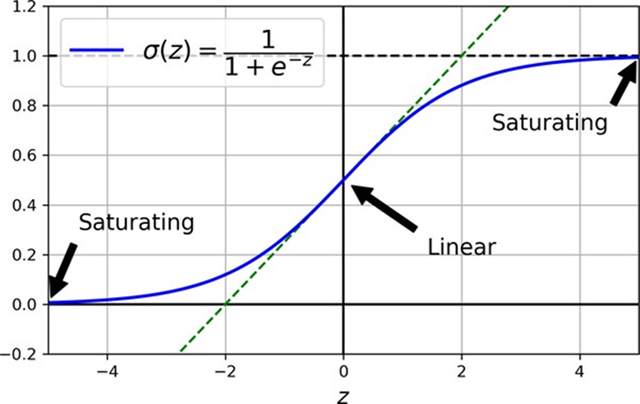
\includegraphics[width=\textwidth,height=0.7\textheight,keepaspectratio]{../machineLearningWeb/Figures/CH11/Hình_11-1}
            \vspace{0.2cm}
            \textit{Hình 11-1: Hàm kích hoạt sigmoid bão hòa ở hai đầu}
        \end{column}
    \end{columns}
\end{frame}

\begin{frame}{Khởi tạo Trọng số Glorot / He (Initialization)}
    \begin{itemize}
        \item Để tín hiệu chảy bình thường trong cả lan truyền xuôi và ngược, \textbf{phương sai} của các tín hiệu đầu ra và đầu vào ở mỗi lớp phải \textbf{bằng nhau}.
        \item Xavier Glorot đề xuất cách khởi tạo các trọng số một cách ngẫu nhiên từ phân phối chuẩn với phương sai: $\sigma^2 = \frac{1}{\text{fan}_{\text{avg}}}$.
        \item Đối với hàm ReLU, Kaiming He đề xuất khởi tạo \textbf{He initialization}: $\sigma^2 = \frac{2}{\text{fan}_{\text{in}}}$.
    \end{itemize}
\end{frame}

\begin{frame}[fragile]{Code: Khởi Tạo Trọng Số trong Keras}
    Theo mặc định, Keras dùng khởi tạo Glorot (với phân phối đều). Để dùng He initialization:
\begin{lstlisting}[language=Python]
import tensorflow as tf
from tensorflow import keras

# Su dung He initialization (thuong ket hop voi ReLU)
dense = keras.layers.Dense(50, activation="relu",
                           kernel_initializer="he_normal")

# Hoac su dung phuong sai do LeCun de xuat (ket hop voi SELU)
dense_lecun = keras.layers.Dense(50, activation="selu",
                           kernel_initializer="lecun_normal")
\end{lstlisting}
\end{frame}

\section{2. Các Hàm Kích Hoạt Nâng Cao}

\begin{frame}{Vấn đề "Dying ReLU"}
    \begin{itemize}
        \item Dù hàm ReLU (Rectified Linear Unit) là tiêu chuẩn vàng, nó có một vấn đề gọi là \textbf{Dying ReLU}.
        \item Nếu trọng số của một nơ-ron ReLU được cập nhật sao cho giá trị tổng tĩnh $z < 0$, nó sẽ luôn trả về 0. 
        \item Đạo hàm của hàm ReLU khi $z < 0$ cũng bằng 0, nghĩa là nơ-ron này sẽ "chết" vĩnh viễn và không bao giờ học lại được nữa.
    \end{itemize}
\end{frame}

\begin{frame}{Hàm Leaky ReLU}
    \begin{columns}
        \begin{column}{0.5\textwidth}
            \begin{itemize}
                \item Giải pháp: $\text{LeakyReLU}_{\alpha}(z) = \max(\alpha z, z)$.
                \item $\alpha$ (thường là 0.01) xác định độ dốc của hàm với các giá trị âm.
                \item "Độ rò rỉ" (leak) này giúp giữ nơ-ron không bị chết hoàn toàn, tạo cơ hội cho gradient được truyền ngược trở lại.
            \end{itemize}
        \end{column}
        \begin{column}{0.5\textwidth}
            \centering
            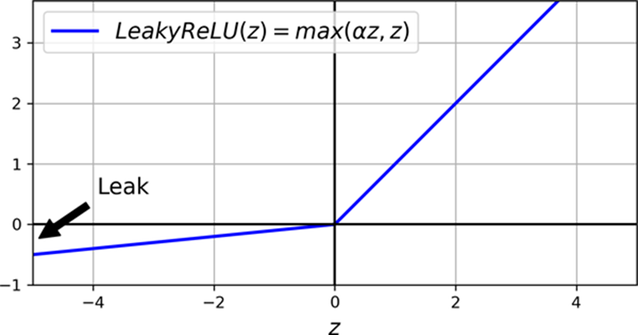
\includegraphics[width=\textwidth,height=0.7\textheight,keepaspectratio]{../machineLearningWeb/Figures/CH11/Hình_11-2}
            \vspace{0.2cm}
            \textit{Hình 11-2: Hàm kích hoạt Leaky ReLU}
        \end{column}
    \end{columns}
\end{frame}

\begin{frame}{ELU và SELU}
    \begin{columns}
        \begin{column}{0.5\textwidth}
            \begin{itemize}
                \item \textbf{ELU (Exponential Linear Unit)}: Mượt mà ở khắp mọi nơi (đạo hàm liên tục tại $z=0$). Cải thiện tốc độ học tập.
                \item \textbf{SELU (Scaled ELU)}: Nếu tất cả các lớp dày đặc sử dụng SELU, mạng sẽ \textbf{tự chuẩn hóa (self-normalize)}, giải quyết vấn đề vanishing gradient.
            \end{itemize}
        \end{column}
        \begin{column}{0.5\textwidth}
            \centering
            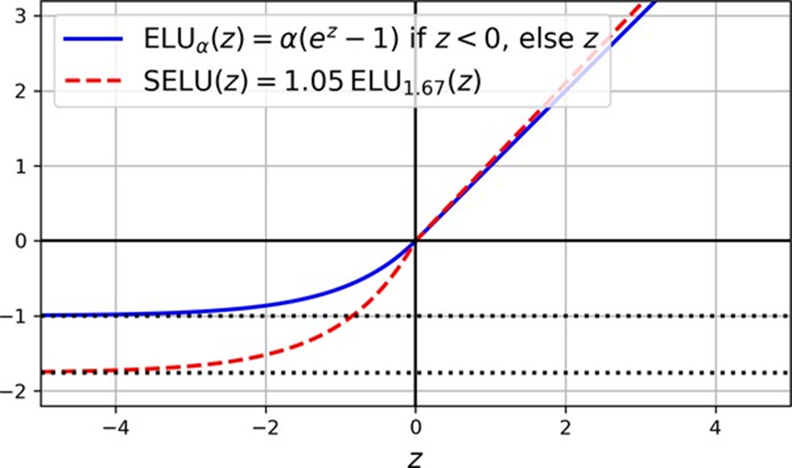
\includegraphics[width=\textwidth,height=0.65\textheight,keepaspectratio]{../machineLearningWeb/Figures/CH11/Hình_11-3}
            \vspace{0.2cm}
            \textit{Hình 11-3: Các hàm kích hoạt ELU và SELU}
        \end{column}
    \end{columns}
\end{frame}

\begin{frame}{GELU, Swish, và Mish}
    \begin{columns}
        \begin{column}{0.5\textwidth}
            \begin{itemize}
                \item Đây là các hàm phức tạp, mượt mà và không đơn điệu (non-monotonic).
                \item \textbf{GELU} (Gaussian Error Linear Unit) vượt trội trong các mạng NLP (như BERT).
                \item \textbf{Swish} do Google Brain đề xuất, tối ưu hơn trong các bài toán Image Recognition sâu.
            \end{itemize}
        \end{column}
        \begin{column}{0.5\textwidth}
            \centering
            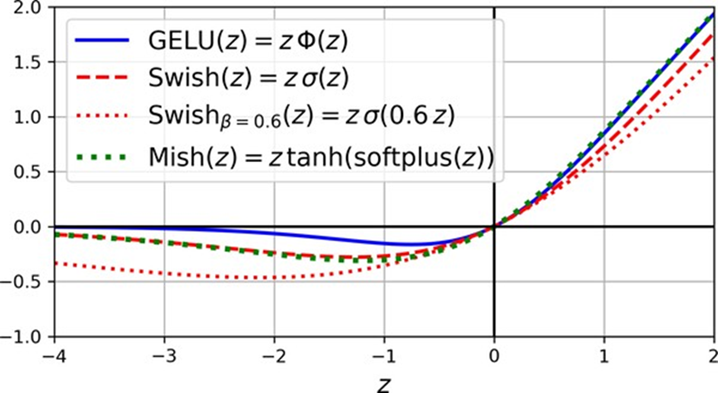
\includegraphics[width=\textwidth,height=0.65\textheight,keepaspectratio]{../machineLearningWeb/Figures/CH11/Hình_11-4}
            \vspace{0.2cm}
            \textit{Hình 11-4: Các hàm kích hoạt GELU, Swish, và Mish}
        \end{column}
    \end{columns}
\end{frame}

\section{3. Batch Normalization và Gradient Clipping}

\begin{frame}{Batch Normalization (Chuẩn hóa Hàng loạt)}
    \begin{itemize}
        \item Khởi tạo He và ELU có thể giảm thiểu vấn đề Vanishing Gradient ở đầu khóa huấn luyện, nhưng nó không đảm bảo không xuất hiện trong quá trình.
        \item Sergey Ioffe và Christian Szegedy (2015) giới thiệu \textbf{Batch Normalization (BN)}.
        \item Lớp BN chuẩn hóa (tính trung bình và độ lệch chuẩn) của các đầu vào tại mỗi lô (mini-batch) một cách độc lập cho từng tính năng.
        \item Sau đó, nó áp dụng thay đổi tỷ lệ (scale) $\gamma$ và độ dịch chuyển (shift) $\beta$ được học qua backpropagation.
    \end{itemize}
\end{frame}

\begin{frame}[fragile]{Code: Thêm Batch Normalization trong Keras}
    \begin{itemize}
        \item Lớp BN thường được thêm trước hoặc sau Hàm kích hoạt của lớp Ẩn.
        \item Kinh nghiệm thực tế cho thấy đặt nó TRƯỚC hàm kích hoạt sẽ hoạt động tốt nhất.
    \end{itemize}
\begin{lstlisting}[language=Python]
model = keras.models.Sequential([
    keras.layers.Flatten(input_shape=[28, 28]),
    keras.layers.BatchNormalization(),
    keras.layers.Dense(300, use_bias=False), # khong can bias vi BN co thuoc tinh dich chuyen(beta)
    keras.layers.BatchNormalization(),
    keras.layers.Activation("relu"),
    keras.layers.Dense(100, use_bias=False),
    keras.layers.BatchNormalization(),
    keras.layers.Activation("relu"),
    keras.layers.Dense(10, activation="softmax")
])
\end{lstlisting}
\end{frame}

\begin{frame}{Hoạt động của BN lúc Inference (Dự đoán)}
    \begin{itemize}
        \item Trong lúc Huấn luyện, BN tính mean, variance của một \textbf{mini-batch}.
        \item Khi Đưa vào ứng dụng (Inference), dữ liệu đến từng cái một, làm sao tính mean và variance?
        \item Giải pháp: BN theo dõi \textbf{moving average} (trung bình động) của mean và variance trên toàn bộ tập huấn luyện. Keras sẽ tự động sử dụng giá trị này khi bạn gọi `model.predict()`.
    \end{itemize}
\end{frame}

\begin{frame}[fragile]{Gradient Clipping}
    \begin{itemize}
        \item Một kỹ thuật phổ biến để giảm bớt vấn đề \textbf{Exploding Gradients} là Cắt (clip) các gradient để chúng không bao giờ vượt quá một ngưỡng (Threshold).
        \item Thường được dùng mạnh mẽ trong Mạng Nơ-ron Hồi quy (RNN).
    \end{itemize}
\begin{lstlisting}[language=Python]
# Cat gradient theo gia tri tuyet doi (-1.0 den 1.0)
optimizer = keras.optimizers.SGD(clipvalue=1.0)
model.compile(loss="mse", optimizer=optimizer)

# Hoac cat theo chuan (Norm) de khong thay doi huong cua vector
optimizer = keras.optimizers.SGD(clipnorm=1.0)
\end{lstlisting}
\end{frame}

\section{4. Tái Sử Dụng Các Lớp (Transfer Learning)}

\begin{frame}{Học Chuyển Giao (Transfer Learning)}
    \begin{columns}
        \begin{column}{0.5\textwidth}
            \begin{itemize}
                \item Sẽ rất lãng phí nếu đào tạo mạng CNN siêu lớn từ con số 0.
                \item Thay vì vậy, ta có thể tìm một Mạng Nơ-ron hiện có thực hiện nhiệm vụ \textbf{tương tự}, giữ lại các lớp dưới (Lower layers), và chỉ thay đổi lớp trên cùng (Output layers).
                \item \textbf{Hình 11-5}: Tái sử dụng các lớp (Freeze) giúp tăng tốc độ đáng kể.
            \end{itemize}
        \end{column}
        \begin{column}{0.5\textwidth}
            \centering
            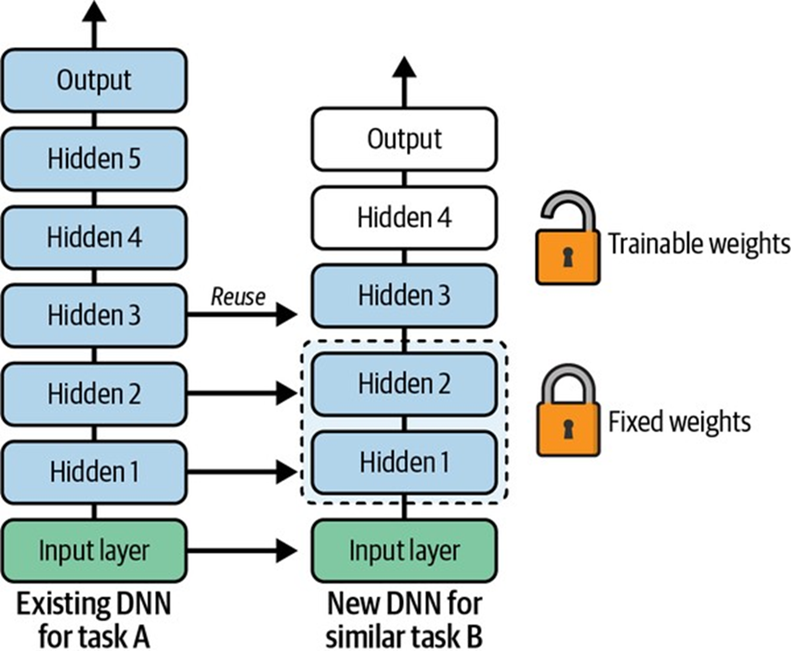
\includegraphics[width=\textwidth,height=0.65\textheight,keepaspectratio]{../machineLearningWeb/Figures/CH11/Hình_11-5}
            \vspace{0.2cm}
            \textit{Hình 11-5: Tái sử dụng các lớp đã được huấn luyện trước}
        \end{column}
    \end{columns}
\end{frame}

\begin{frame}[fragile]{Code: Tái sử dụng mô hình trong Keras}
\begin{lstlisting}[language=Python]
# Tai mot mo hinh da huan luyen (Model A)
model_A = keras.models.load_model("my_model_A.h5")

# Tao Model B dua tren cac lop cua Model A (tru lop cuoi)
model_B_on_A = keras.models.Sequential(model_A.layers[:-1])
model_B_on_A.add(keras.layers.Dense(1, activation="sigmoid"))

# Dong bang (Freeze) cac lop cu
for layer in model_B_on_A.layers[:-1]:
    layer.trainable = False

# Huan luyen vai epoch de cap nhat lop cuoi
model_B_on_A.compile(loss="binary_crossentropy", optimizer="sgd")
model_B_on_A.fit(X_train_B, y_train_B, epochs=4)
\end{lstlisting}
\end{frame}

\begin{frame}{Huấn Luyện Không Giám Sát (Unsupervised Pretraining)}
    \begin{columns}
        \begin{column}{0.5\textwidth}
            \begin{itemize}
                \item Điều gì xảy ra nếu bạn có quá ít dữ liệu gắn nhãn (Labeled data)?
                \item Bạn có thể đào tạo trước bằng Học không giám sát (như Autoencoders hoặc RBMs).
                \item Sau đó chèn thêm lớp phân loại và huấn luyện có giám sát.
                \item \textbf{Hình 11-6}: Các mô hình NLP ngôn ngữ lớn như GPT và BERT cũng là một dạng Unsupervised Pretraining khổng lồ!
            \end{itemize}
        \end{column}
        \begin{column}{0.5\textwidth}
            \centering
            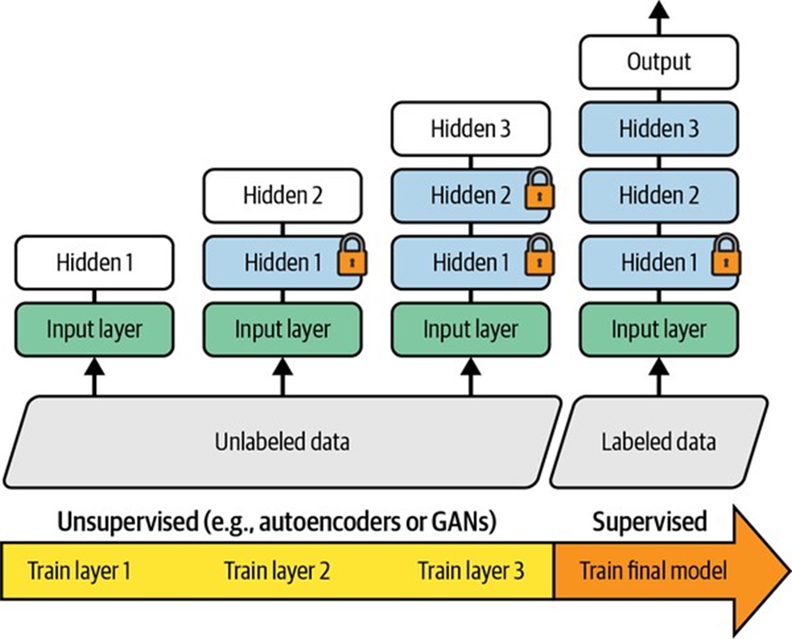
\includegraphics[width=\textwidth,height=0.65\textheight,keepaspectratio]{../machineLearningWeb/Figures/CH11/Hình_11-6}
            \vspace{0.2cm}
            \textit{Hình 11-6: Học chuyển giao từ huấn luyện không giám sát}
        \end{column}
    \end{columns}
\end{frame}

\section{5. Các Trình Tối Ưu Hóa Tốc Độ Học (Fast Optimizers)}

\begin{frame}{Giới thiệu các Optimizer (Trình tối ưu hóa)}
    \begin{itemize}
        \item SGD (Stochastic Gradient Descent) cơ bản hoạt động ổn định nhưng \textbf{cực kỳ chậm}.
        \item Các nhà khoa học đã phát triển ra các thuật toán Tối ưu hóa có khả năng chạy nhanh gấp 10-100 lần.
        \item Các Optimizer nổi tiếng:
        \begin{enumerate}
            \item Momentum Optimization
            \item Nesterov Accelerated Gradient (NAG)
            \item AdaGrad
            \item RMSProp
            \item Adam / Nadam
        \end{enumerate}
    \end{itemize}
\end{frame}

\begin{frame}{Tối ưu hóa Bằng Động Lượng (Momentum)}
    \begin{itemize}
        \item SGD cập nhật trọng số dựa hoàn toàn trên \textbf{gradient tại thời điểm hiện tại}. Nó giống như đi xuống núi nhưng rẽ ngoặt theo góc dốc ngay dưới chân.
        \item Momentum quan tâm đến \textbf{các gradient trước đó}. Giống như thả một quả bóng bowling xuống bề mặt trơn: quả bóng sẽ liên tục \textbf{tăng tốc} (động lượng lớn).
        \item Cập nhật công thức:
        \begin{align*}
            m &\leftarrow \beta m - \eta \nabla_\theta J(\theta) \\
            \theta &\leftarrow \theta + m
        \end{align*}
        \item Keras: \texttt{keras.optimizers.SGD(learning\_rate=0.001, momentum=0.9)}
    \end{itemize}
\end{frame}

\begin{frame}{Nesterov Accelerated Gradient (NAG)}
    \begin{columns}
        \begin{column}{0.5\textwidth}
            \begin{itemize}
                \item Biến thể của Momentum.
                \item Thay vì tính đạo hàm tại vị trí hiện tại $\theta$, NAG tính đạo hàm ở bước \textbf{tiến tới (Look-ahead)} một khoảng $\beta m$.
                \item Điều này giúp thuật toán "đạp phanh" kịp thời khi đến gần đáy lũng.
                \item \textbf{Hình 11-7} so sánh Momentum thông thường (màu xanh lam) và NAG (màu đỏ).
            \end{itemize}
        \end{column}
        \begin{column}{0.5\textwidth}
            \centering
            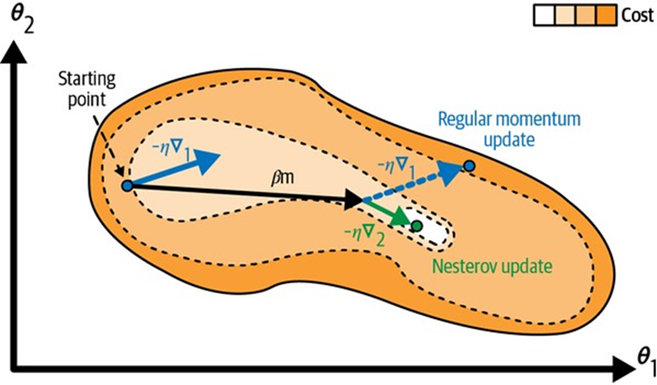
\includegraphics[width=\textwidth,height=0.6\textheight,keepaspectratio]{../machineLearningWeb/Figures/CH11/Hình_11-7}
            \vspace{0.2cm}
            \textit{Hình 11-7: So sánh Momentum thông thường và Nesterov}
        \end{column}
    \end{columns}
\end{frame}

\begin{frame}{AdaGrad}
    \begin{columns}
        \begin{column}{0.5\textwidth}
            \begin{itemize}
                \item Trong các bài toán có nhiều chiều (dimensions) bị thon dài (elongated bowl).
                \item Thuật toán AdaGrad tự động \textbf{làm giảm tốc độ học} dọc theo các chiều có độ dốc quá cao (steep dimensions).
                \item \textbf{Hình 11-8}: AdaGrad đi thẳng tới đích rành mạch hơn thay vì "ngoằn ngoèo" như SGD.
                \item Lưu ý: AdaGrad bị dừng quá sớm khi dùng cho Neural Networks, do vậy chỉ dùng trong hồi quy tuyến tính.
            \end{itemize}
        \end{column}
        \begin{column}{0.5\textwidth}
            \centering
            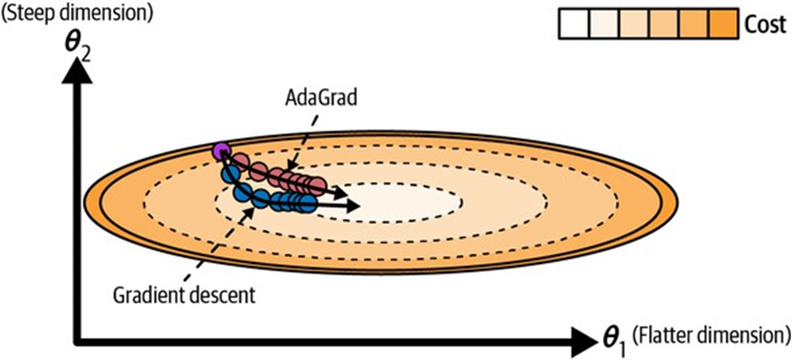
\includegraphics[width=\textwidth,height=0.65\textheight,keepaspectratio]{../machineLearningWeb/Figures/CH11/Hình_11-8}
            \vspace{0.2cm}
            \textit{Hình 11-8: So sánh AdaGrad và Gradient Descent}
        \end{column}
    \end{columns}
\end{frame}

\begin{frame}[fragile]{RMSProp và Adam}
    \begin{itemize}
        \item \textbf{RMSProp}: Sửa chữa nhược điểm của AdaGrad bằng cách chỉ xem xét các gradient gần đây (thay vì tích lũy từ đầu). Rất phổ biến trước khi Adam ra đời.
        \item \textbf{Adam (Adaptive Moment Estimation)}: Kết hợp tính chất tuyệt vời của Momentum (tích lũy gradient) và RMSProp (tích lũy bình phương gradient).
        \item Adam là Optimizer "mặc định" và thành công vang dội nhất hiện nay cho Mạng Nơ-ron.
    \end{itemize}
\begin{lstlisting}[language=Python]
# Hien tai Optimizer xin so va de dung nhat la Adam
optimizer = keras.optimizers.Adam(learning_rate=0.001, beta_1=0.9, beta_2=0.999)
\end{lstlisting}
\end{frame}

\section{6. Lịch Trình Tốc Độ Học (Learning Rate Scheduling)}

\begin{frame}{Vấn đề của Tốc Độ Học Cố Định}
    \begin{columns}
        \begin{column}{0.5\textwidth}
            \begin{itemize}
                \item Tốc độ học (Learning Rate - $\eta$) là siêu tham số quan trọng nhất.
                \item Quá lớn: mô hình phân kỳ. Quá nhỏ: mất quá nhiều thời gian hội tụ.
                \item \textbf{Hình 11-9}: Nếu ta bắt đầu lớn (để tiến nhanh), sau đó giảm dần (để hội tụ chính xác), ta sẽ đạt kết quả tối ưu nhất trong thời gian ngắn nhất!
            \end{itemize}
        \end{column}
        \begin{column}{0.5\textwidth}
            \centering
            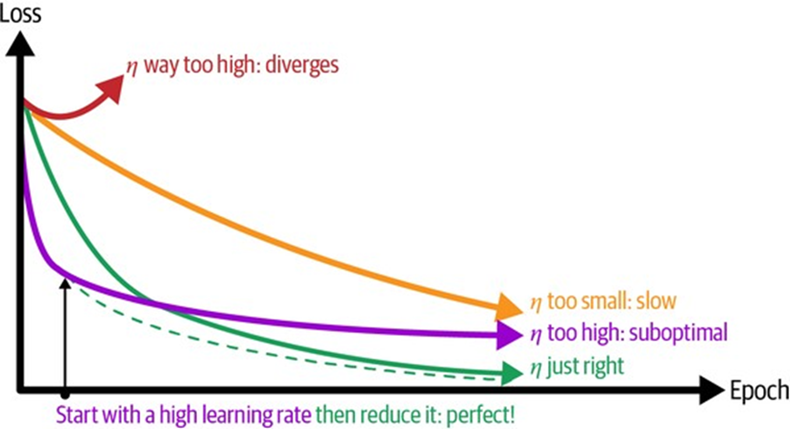
\includegraphics[width=\textwidth,height=0.65\textheight,keepaspectratio]{../machineLearningWeb/Figures/CH11/Hình_11-9}
            \vspace{0.2cm}
            \textit{Hình 11-9: Lịch trình tốc độ học}
        \end{column}
    \end{columns}
\end{frame}

\begin{frame}[fragile]{Code: Power Scheduling trong Keras}
    \begin{itemize}
        \item Lập lịch theo hàm lũy thừa: $\eta(t) = \eta_0 / (1 + t/s)^c$.
        \item Keras thực hiện cực kì dễ thông qua tham số `decay` (Keras phiên bản cũ) hoặc `InverseTimeDecay`.
    \end{itemize}
\begin{lstlisting}[language=Python]
lr_schedule = keras.optimizers.schedules.InverseTimeDecay(
    initial_learning_rate=0.01,
    decay_steps=10000,
    decay_rate=1.0)
    
optimizer = keras.optimizers.SGD(learning_rate=lr_schedule)
\end{lstlisting}
\end{frame}

\begin{frame}[fragile]{Code: Performance Scheduling}
    \begin{itemize}
        \item Giảm tốc độ học một nửa khi hàm lỗi (validation error) ngưng giảm.
        \item Trong Keras, sử dụng Callback \texttt{ReduceLROnPlateau}.
    \end{itemize}
\begin{lstlisting}[language=Python]
lr_scheduler = keras.callbacks.ReduceLROnPlateau(
    factor=0.5, # giam mot nua
    patience=5) # neu sau 5 epoch khong giam loi, thi giam LR

model.fit(X_train, y_train, epochs=50,
          validation_data=(X_valid, y_valid),
          callbacks=[lr_scheduler])
\end{lstlisting}
\end{frame}

\section{7. Kỹ Thuật Chính Quy Hóa (Regularization)}

\begin{frame}{Tổng Quan Các Phương Pháp Chính Quy Hóa}
    \begin{itemize}
        \item "Với hàng tỷ trọng số tự do, mạng nơ-ron sâu có thể học rất tốt, thậm chí nhớ luôn cả nhiễu trong dữ liệu."
        \item Đây chính là \textbf{Overfitting} (Quá khớp).
        \item Các kỹ thuật phổ biến để khắc phục:
        \begin{enumerate}
            \item L1 và L2 Regularization (Kìm hãm trọng số lớn)
            \item Dropout (Loại bỏ ngẫu nhiên)
            \item Max-Norm (Giới hạn chuẩn vector trọng số)
            \item Data Augmentation (Tăng cường dữ liệu bằng biến đổi hình ảnh/âm thanh)
        \end{enumerate}
    \end{itemize}
\end{frame}

\begin{frame}[fragile]{L1 và L2 Regularization}
    \begin{itemize}
        \item Cộng thêm hình phạt (penalty) bằng độ lớn của trọng số (Weights) vào hàm Mất Mát (Loss Function).
        \item Có thể thiết lập dễ dàng trong Keras layers:
    \end{itemize}
\begin{lstlisting}[language=Python]
# Ap dung l2 regularization voi he so 0.01
layer = keras.layers.Dense(100, activation="elu",
                           kernel_initializer="he_normal",
                           kernel_regularizer=keras.regularizers.l2(0.01))
\end{lstlisting}
    \begin{itemize}
        \item Để mã sạch hơn (do lặp lại nhiều lần), bạn có thể dùng tính năng `functools.partial`.
    \end{itemize}
\end{frame}

\begin{frame}{Dropout - "Liều Thuốc Mê" Cho Nơ-ron}
    \begin{columns}
        \begin{column}{0.5\textwidth}
            \begin{itemize}
                \item G. E. Hinton (2012) giới thiệu thuật toán đơn giản một cách vô lý nhưng cực kỳ thành công: \textbf{Dropout}.
                \item Tại mỗi lượt huấn luyện, mỗi nơ-ron có xác suất $p$ (thường từ 10\% đến 50\%) bị "ngắt" tạm thời.
                \item Các nơ-ron không thể phụ thuộc vào đồng nghiệp kế bên mà tự thân vận động trích xuất các đặc trưng hữu ích nhất.
                \item \textbf{Hình 11-10}: Minh họa mạng áp dụng kỹ thuật Dropout.
            \end{itemize}
        \end{column}
        \begin{column}{0.5\textwidth}
            \centering
            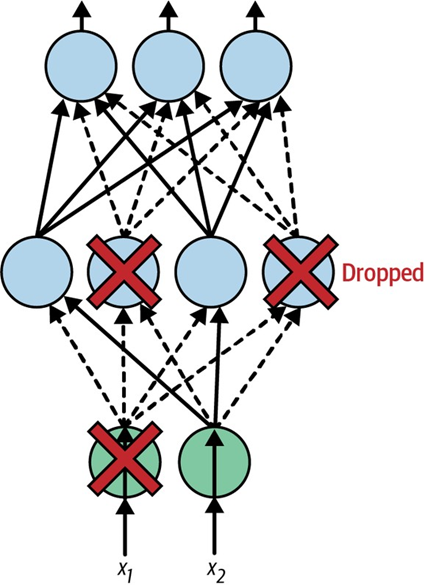
\includegraphics[width=\textwidth,height=0.65\textheight,keepaspectratio]{../machineLearningWeb/Figures/CH11/Hình_11-10}
            \vspace{0.2cm}
            \textit{Hình 11-10: Với chính quy hóa dropout, một số nơ-ron bị tắt ngẫu nhiên}
        \end{column}
    \end{columns}
\end{frame}

\begin{frame}[fragile]{Sử dụng Dropout trong Keras}
    \begin{itemize}
        \item \textbf{Quan trọng}: Khi Dropout huấn luyện, chỉ còn khoảng một nửa số nơ-ron tham gia dự đoán. Vì vậy, trong giai đoạn \textbf{Test/Inference}, ta PHẢI nhân giá trị với xác suất giữ lại để cân bằng. (Keras tự động xử lý việc này).
    \end{itemize}
\begin{lstlisting}[language=Python]
model = keras.models.Sequential([
    keras.layers.Flatten(input_shape=[28, 28]),
    keras.layers.Dropout(rate=0.2), # ngat 20% no-ron
    keras.layers.Dense(300, activation="elu", kernel_initializer="he_normal"),
    keras.layers.Dropout(rate=0.2),
    keras.layers.Dense(100, activation="elu", kernel_initializer="he_normal"),
    keras.layers.Dropout(rate=0.2),
    keras.layers.Dense(10, activation="softmax")
])
\end{lstlisting}
\end{frame}

\begin{frame}{Monte Carlo (MC) Dropout}
    \begin{itemize}
        \item Y. Gal và Z. Ghahramani (2016) chỉ ra rằng mạng nơ-ron sử dụng Dropout tương đương toán học với quá trình xấp xỉ suy luận Bayes (Bayesian inference).
        \item Cụ thể, \textbf{MC Dropout} bật Dropout ngay cả trong giai đoạn Inference (Dự đoán).
        \item Khi ta thực hiện dự đoán 100 lần trên cùng 1 mẫu, ta sẽ nhận được 100 kết quả dự đoán (xác suất) khác nhau do mỗi lần mạng lại tắt đi một số nơ-ron ngẫu nhiên.
        \item Tính trung bình và phương sai của các dự đoán đó sẽ cho ta một độ tin cậy vô cùng chính xác!
    \end{itemize}
\end{frame}

\begin{frame}[fragile]{Code: Thực Hiện MC Dropout Bằng Keras}
\begin{lstlisting}[language=Python]
import numpy as np

# Bat tinh nang Training = True ben trong lop Dropout ke ca khi du doan
y_probas = np.stack([model(X_test_scaled, training=True)
                     for sample in range(100)])
y_proba = y_probas.mean(axis=0)
y_std = y_probas.std(axis=0) # Do bat dinh (Uncertainty)
\end{lstlisting}
\end{frame}

\begin{frame}[fragile]{Alpha Dropout}
    \begin{itemize}
        \item Nếu bạn sử dụng hàm kích hoạt \textbf{SELU} để mạng tự chuẩn hóa (self-normalize).
        \item Thì sử dụng Dropout thông thường sẽ phá hủy sự tự chuẩn hóa đó!
        \item Hãy sử dụng \texttt{AlphaDropout} - một biến thể của Dropout bảo toàn được giá trị trung bình và phương sai.
    \end{itemize}
\begin{lstlisting}[language=Python]
model.add(keras.layers.AlphaDropout(rate=0.2))
\end{lstlisting}
\end{frame}

\begin{frame}{Max-Norm Regularization}
    \begin{itemize}
        \item Hạn chế (clamp) không cho chuẩn l2 (Norm 2) của vector trọng số của mỗi nơ-ron vượt quá một giá trị lớn nhất $r$.
        \item Cụ thể: $\|\mathbf{w}\|_2 \le r$.
        \item Nếu vượt quá, trọng số sẽ được chia tỉ lệ: $\mathbf{w} \leftarrow \mathbf{w} \frac{r}{\|\mathbf{w}\|_2}$.
        \item Max-norm kết hợp rất tốt với Dropout để kìm hãm sự tăng trưởng vô hạn của các trọng số.
    \end{itemize}
\end{frame}

\begin{frame}[fragile]{Code: Max-Norm Trong Keras}
\begin{lstlisting}[language=Python]
dense = keras.layers.Dense(100, activation="elu",
                           kernel_initializer="he_normal",
                           kernel_constraint=keras.constraints.max_norm(1.))
\end{lstlisting}
\end{frame}

\begin{frame}{Tối ưu hóa RMSProp}
    \begin{itemize}
        \item AdaGrad đôi khi giảm tốc độ học quá mức và dừng sớm trước khi đến mục tiêu cực trị toàn cục (global optimum).
        \item RMSProp là phiên bản nâng cấp của AdaGrad, giải quyết việc dừng sớm bằng cách chỉ tích lũy bình phương của các gradient \textbf{gần đây nhất} thay vì tất cả gradient từ đầu thuật toán.
        \item Thuật toán này sử dụng tốc độ phân rã lũy thừa $\beta$ (exponential decay).
    \end{itemize}
\end{frame}

\begin{frame}[fragile]{Code: Tối Ưu Hóa RMSProp Keras}
\begin{lstlisting}[language=Python]
# Tinh chinh toc do doc bang RMSprop
optimizer = keras.optimizers.RMSprop(learning_rate=0.001, rho=0.9)
\end{lstlisting}
    \begin{itemize}
        \item Tham số `rho` tương ứng với $\beta$ trong công thức lý thuyết (thường đặt là 0.9).
        \item Ngoại trừ những kiến trúc cực kỳ phức tạp, RMSProp gần như luôn hoạt động tốt hơn hẳn so với AdaGrad.
    \end{itemize}
\end{frame}

\begin{frame}{Adam, Nadam \& AdamW}
    \begin{itemize}
        \item \textbf{Adam} kết hợp Momentum (theo dõi động lượng) và RMSProp (theo dõi bình phương gradient).
        \item \textbf{Nadam} là Adam cộng với kỹ thuật Nesterov Accelerated Gradient (NAG), cho tốc độ hội tụ nhanh hơn một chút.
        \item \textbf{AdamW} là Adam kết hợp với kỹ thuật điều chuẩn phân rã trọng số (weight decay regularization) thực thụ, thường dùng cho mạng biến áp (Transformers).
    \end{itemize}
\end{frame}

\begin{frame}{Tóm Tắt Lựa Chọn Các Kỹ Thuật (Phần 1)}
    \begin{table}
        \centering
        \small
        \begin{tabular}{ll}
        \hline
        \textbf{Thành phần}           & \textbf{Lựa chọn mặc định}                 \\ \hline
        Cấu hình khởi tạo (Init)      & Khởi tạo He (He initialization)            \\
        Hàm kích hoạt (Activation)    & ELU hoặc GELU (hoặc Swish)                 \\
        Chuẩn hóa (Normalization)     & Mạng nông/sâu: Batch Normalization (BN)    \\
        Chống quá khớp (Regularize)   & Early Stopping + Dropout                   \\
        Trình tối ưu hóa (Optimizer)  & Nadam hoặc AdamW (kèm Warmup)              \\
        Lịch trình tốc độ học         & Performance Scheduling (hoặc One Cycle)    \\ \hline
        \end{tabular}
    \end{table}
\end{frame}

\begin{frame}{Tóm Tắt Lựa Chọn Nếu Tự Chuẩn Hóa (Phần 2)}
    Nếu bạn xây dựng Mạng dày đặc (Dense) và muốn nó tự chuẩn hóa (Self-Normalizing):
    \begin{table}
        \centering
        \small
        \begin{tabular}{ll}
        \hline
        \textbf{Thành phần}           & \textbf{Cấu hình Mạng Tự Chuẩn Hóa}        \\ \hline
        Cấu hình khởi tạo (Init)      & Khởi tạo LeCun                             \\
        Hàm kích hoạt (Activation)    & SELU                                       \\
        Chuẩn hóa (Normalization)     & Không cần (tự thân chuẩn hóa)              \\
        Chống quá khớp (Regularize)   & Alpha Dropout                              \\ \hline
        \end{tabular}
    \end{table}
\end{frame}

\begin{frame}{Các Vấn Đề Thực Tế Khác}
    \begin{itemize}
        \item Nếu bạn làm việc trên các mô hình Thưa (Sparse models), hãy dùng $L_1$ Regularization.
        \item Nếu thiết bị của bạn cần tốc độ phản hồi cực nhanh (low latency) khi ứng dụng thực tế (Inference), hãy loại bỏ Batch Normalization bằng cách hợp nhất (fuse) các tham số vào lớp trước đó, và dùng Leaky ReLU.
        \item Luôn tận dụng tài nguyên có sẵn: Đừng quên Transfer Learning!
    \end{itemize}
\end{frame}

\begin{frame}{Tổng Kết Chương 11}
    \begin{itemize}
        \item Chúng ta đã giải quyết rốt ráo việc \textbf{Huấn Luyện Các Mạng Khổng Lồ} mà không để rơi vào tình trạng Vanishing Gradient.
        \item \textbf{Khởi tạo He} kết hợp hàm \textbf{ELU / GELU} là lựa chọn tiêu chuẩn.
        \item Củng cố bằng \textbf{Batch Normalization}.
        \item Sử dụng \textbf{Adam Optimizer} với Lịch trình Học Tập (Learning Rate Schedule).
        \item Và đương nhiên, chống Overfitting hiệu quả bằng \textbf{Dropout}.
    \end{itemize}
\end{frame}

\end{document}
